Nous voulons explorer l'hypothèse selon laquelle les codes longs
comporteraient plus de warnings à la compilation que les courts. Nous
avons commencé par séparer notre table en deux, l'une pour les
programmes au nombre de lignes de code inférieur à la médiane et
l'autre pour les autres programmes. 

Nous avons ensuite effectué trois tests de Mann-Whitney, un pour chaque
type de warning (Clang, MinorWarning de gcc, MajorWarning de gcc),
avec pour hypothèse nulle ``Il n'y a pas de différence significative
du nombre moyen de warnings à la compilation entre les programmes de
longueurs supérieures et inférieures à la médiane.''. Nous avons pour
cela encore une fois supposé que les échantillons considérés suivaient
une loi normale de variance identique. Lors du test, nous avons passé
\lstinline{alternative = "less"} en argument à la fonction
\lstinline{wilcox.test}, cela correspond au fait que nous nous attendons à
ce que le nombre de warnings soit supérieur pour pour les programmes
long.

Pour les warnings Clang, la p-value retournée par le test est de
0.0006216, au risque d'erreur 5\%, nous pouvons donc rejeter
l'hypothèse nulle. Nous en concluons que le nombre moyen de warnings Clang
est supérieur pour les programmes longs.

Pour les warnings gcc, la p-value retournée par le test est de 0.7749
et 0.08464 pour les warning mineurs et majeurs respectivement. Au
risque d'erreur 5\%, nous ne pouvons donc pas rejeter l'hypothèse
nulle. Nous en concluons que le nombre moyen de warnings gcc n'est pas
significativement supérieur pour les programmes longs.

Le test de Mann-Whitney étant un test de comparaison de moyennes, nous
avons voulu approfondir le lien entre le nombre de warnings Clang et la
taille des programmes. Pour cela, nous avons décider de faire un test de
corrélation entre ces deux grandeurs. Nous avons pour cela effectué un
test paramétrique de corrélation de Pearson avec la fonction
\emph{cor.test}. Ce test nécéssite que les données suivent une loi
normale, cette condition étant ici discutable, nous avons aussi
effectué un test non-paramétrique : le test de
corrélation de Spearman, disponible avec la même fonction. 

Le test de Pearson renvoie une p-value de 0.03095, et le test de
Spearman de 0.001907. Nous pouvons donc affirmer au risque d'erreur 5 \%
que le nombre de lignes de codes et le nombre de warnings Clang sont
corrélés.

Nous avons donc généré un graphique représentant le nombre de warnings
Clang en fonction du nombre de lignes de code, sur lequel nous avons
tracé une droite de régression linéaire (figure \ref{fig:clang_lin}).

\begin{figure}[h]
  \centering
  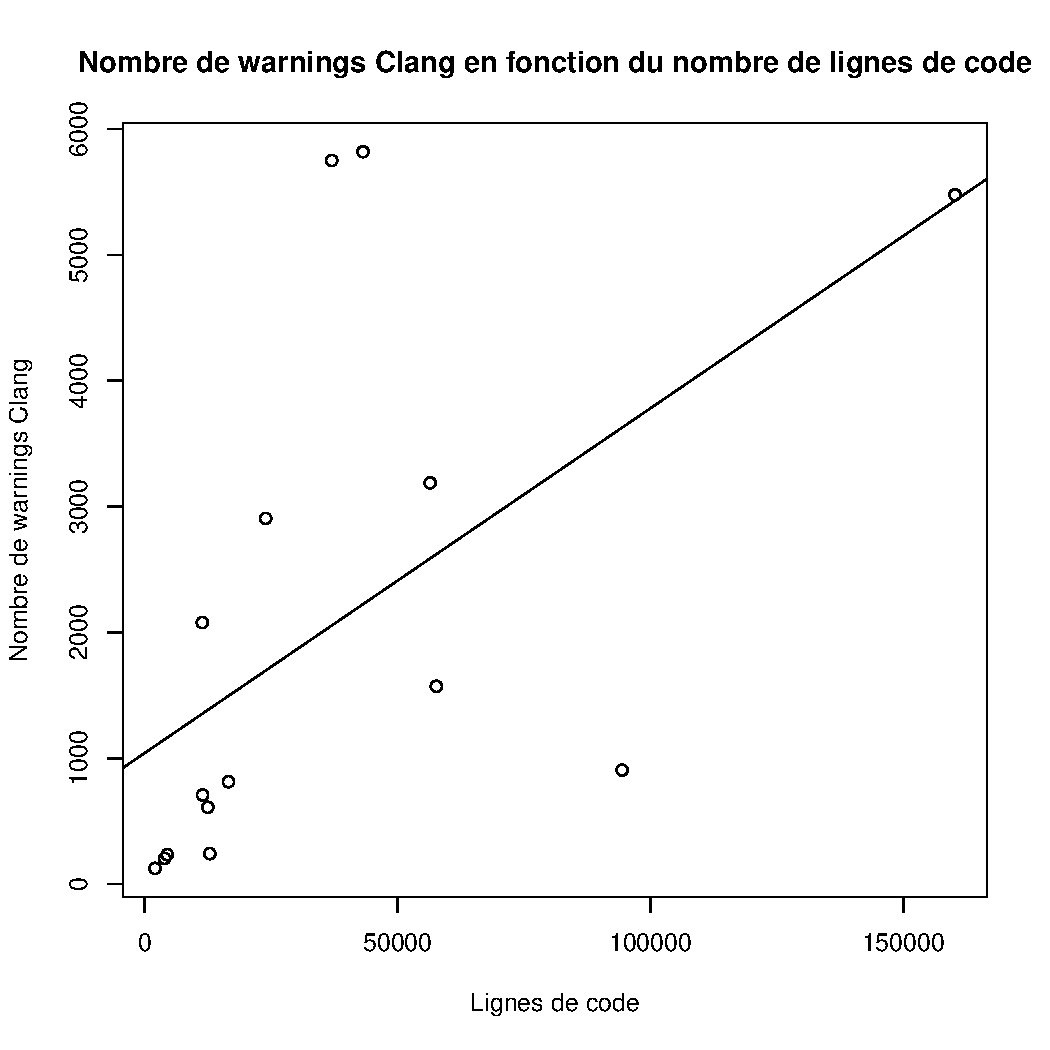
\includegraphics[width=.48\textwidth]{figures/clang_lin.pdf}
  \caption{}\label{fig:clang_lin}
\end{figure}
